\documentclass[a4paper, times, 10pt,twocolumn]{article}
\usepackage[top=4.9cm,bottom=3.7cm,left=1.5cm,right=1.5cm]{geometry}
% \usepackage{ctex}
\usepackage{ICMLC}
\usepackage{times}
\usepackage{graphicx}
\usepackage{indentfirst}
\usepackage{latexsym}
\usepackage{amsfonts}
\usepackage{amsmath}
\usepackage{amssymb}

%option
%\newtheorem{definition}{Definition}
%\newtheorem{example}{Example}
%\renewcommand{\tablename}{TABLE}
%\renewcommand{\figurename}{FIGURE}
\usepackage[margin=8pt,font=footnotesize,labelfont=bf,labelsep=period
]{caption}

%balance package is an option
%\usepackage{balance}
%\balance
%-------------------------------------------------------------------------

\pdfpagewidth=\paperwidth
\pdfpageheight=\paperheight
\pagestyle{empty}

%-------------------------------------------------------------------------
\begin{document}

\title{A Multi-stage Cascaded Encoder-decoder Framework for CT-to-PET Image Conversion in Lung Imaging}  % The title should be in Upper case

\author{\bf{\normalsize{Xiaoyu Deng${^1}{^*}$, Kouki Nagamune${^2}$, Hiroki Takada${^1}$}}\\ % The author should be in Upper case
	\\
	\normalsize{$^1$University of Fukui, 3-9-1 Bunkyo, Fukui, 910-0017, Japan}\\
	\normalsize{$^2$University of Hyogo, 2167 Shosha, Himeji, Hyogo, 671-2280, Japan} \\
	\normalsize{$^*$Corresponding author, E-MAIL: xyxy.jp@gmail.com}\\
	\\}


\maketitle \thispagestyle{empty}

\begin{abstract}
	{
		Deep learning architectures have profoundly impacted medical image processing by effectively preserving essential spatial information crucial for accurate segmentation tasks. Despite enhancements through depth expansion, increased channels, refined skip connections, or integration of attention-based modules like Transformers, these approaches typically heighten computational complexity and limit practical efficiency.

		This study introduces a multi-stage cascaded framework specifically designed for CT-to-PET image conversion, employing sequentially linked, simplified encoder-decoder modules to balance simplicity and computational efficiency. Using publicly available lung cancer PET-CT datasets, experimental results indicate progressive enhancements in image reconstruction quality across cascade stages. Quantitative metrics, including Structural Similarity Index Measure, Peak Signal-to-Noise Ratio, and Mean Absolute Error, reflect notable improvements, with optimal results reaching an SSIM of 0.9291 and a PSNR of 28.8474 dB.

		Nevertheless, visual inspection reveals residual artifacts from transposed convolution operations, highlighting the limitations of pixel-level metrics alone in capturing perceptual image quality. Hence, the proposed cascaded framework demonstrates significant potential for clinical PET image synthesis from CT scans, emphasizing future integration of comprehensive visual quality and expert evaluations.
	}
\end{abstract}
%-------------------------------------------------------------------------
\begin{keywords}
	{Cross-modal medical image synthesis, CT-to-PET, Cascaded generators, Generative adversarial networks, Multimodal imaging}
\end{keywords}

%-------------------------------------------------------------------------
\Section{Introduction}
Encoder-decoder architectures exemplified by U-Net, have revolutionized medical image processing due to their capability to effectively capture and reconstruct complex spatial features. Originally developed for segmentation, U-Net achieves superior performance through a distinctive symmetrical structure composed of an encoding (contracting) pathway and a decoding (expansive) pathway. This dual-path approach, combined with strategically placed skip connections, significantly enhances the accuracy of spatial information retention during the upsampling process, a crucial attribute for accurately delineating anatomical structures in medical imaging.

Increasing the scale of U-Net models can involve deepening the network, increasing the number of feature map channels, improving skip connection structures, and incorporating attention modules like Transformers. While these enhancements can improve performance, they also increase model complexity and computational demands, often leading to performance bottlenecks. In this research, multiple simple encoder-decoder structures are used to construct a generative network, verifying the performance of multi-stage models in medical image generation tasks.

The main contributions of this paper include proposing a multi-stage cascaded extension framework, constructing multiple multi-stage cascade models with simple encoder-decoder modules for CT-to-PET image conversion tasks, validating the effectiveness of this framework through experiments, and presenting performance metrics across various stages. The specific contributions are:

Proposing a multi-stage cascaded framework utilizing multiple simple encoder-decoder models for lung CT-to-PET image conversion tasks without altering individual encoder-decoder structures.

Experimentally validating the effectiveness of the proposed framework on publicly available paired PET-CT datasets, showcasing the performance of U-Net models at each stage, and monitoring various training and testing metrics.

Visually comparing images generated by different cascade models against real images to explore the effect of cascading on visual quality.

%-------------------------------------------------------------------------
\section{Related Works}
Since the introduction of U-Net by Olaf et al. \cite{navab_u-net_2015}, it has been extensively employed due to its structural advantages and excellent performance in applications such as image denoising, medical image registration, and attenuation correction. It has also been applied in various other segmentation tasks including lesion segmentation and facial image restoration.

Armanious et al. \cite{armanious_medgan_2020} proposed an end-to-end GAN-based framework for medical image-to-image translation, demonstrating its performance in PET-CT translation, MR motion artifact correction, and PET denoising tasks. Singh et al. \cite{singh_automated_2023} presented a U-Net-based automated medical image registration method, employing GAN to generate pseudo-CT images from non-attenuation-corrected PET images, enhancing coronary angiography registration accuracy. Liu et al. \cite{liu_deep_2018} developed a method for generating pseudo-CT images for attenuation correction from single non-attenuation-corrected 18F-FDG PET images. Du et al. \cite{du_medical_2020} reviewed six U-Net-based methods for medical image segmentation, including lung nodules, cardiac, and brain segmentation tasks. Zeng et al. \cite{zeng_swin-casunet_2022} used a two-stage cascaded U-Net for facial image restoration, indicating potential advantages of multi-stage U-Net models for image generation tasks. Singh and Liu applied models with fine-tuned modules in medical image registration and attenuation correction, achieving notable results. While Armanious and Zeng utilized cascaded U-Net structures, multi-stage cascaded U-Net models for medical image generation remain underexplored. This study evaluates multi-stage cascaded U-Net models for CT-to-PET image conversion tasks using several metrics.

The Structural Similarity Index \cite{zhou_wang_image_2004} (SSIM) measures structural similarity between two images, considering luminance, contrast, and structural information, ranging from -1 to 1, with 1 indicating identical images. The Multi-scale SSIM (MS-SSIM) extends SSIM across multiple scales, better assessing image quality across varying resolutions. Peak Signal-to-Noise Ratio \cite{hore_image_2010} (PSNR) measures image reconstruction quality by comparing original and processed images, widely used in signal processing applications. Mean Absolute Error\cite{chai_root_2014} (MAE) computes the average pixel intensity difference between reconstructed and original images, insensitive to outliers compared to Mean Squared Error (MSE), thus selected as an evaluation metric given pixel scaling between 0 and 1 in PyTorch frameworks.
%-------------------------------------------------------------------------
% % TODO: \usepackage{graphicx} required
\begin{figure*}[t!]
	\centering
	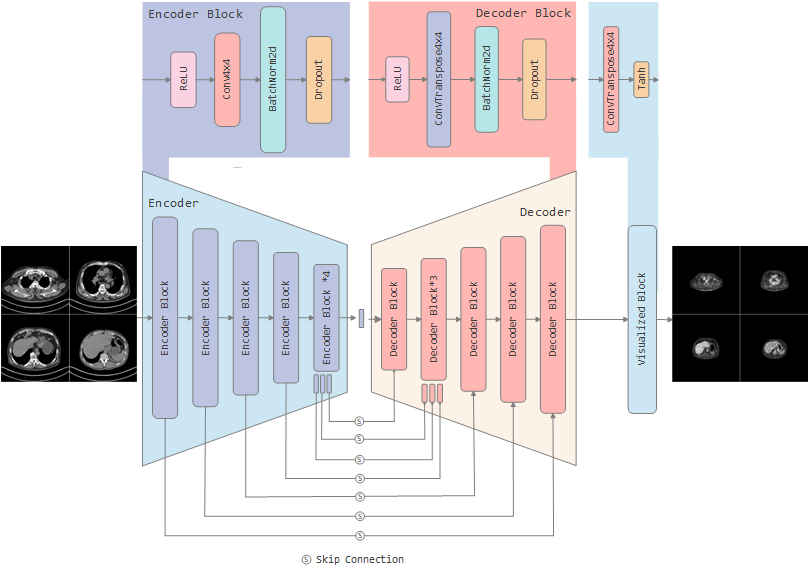
\includegraphics[width=1.0\linewidth]{figures/lung/Encoder-Decoder-5layer-250406}
	\caption[architecture]{Schematic Diagram of Data Flow Within the Model. The PET image is shown on the left, and the CT image on the right. The blue modules correspond to the encoder architecture, while the orange modules represent the decoder architecture. The upper portion of the figure illustrates the fundamental structures of the encoder blocks, decoder blocks, and visualization blocks. The connections in the lower portion indicate the skip connections.}
	\label{fig:Encoder_Decoder_Pair}
\end{figure*}

\section{Method}
The proposed methods comprises encoder, decoder, and visualization modules. The encoder extracts image features, the decoder reconstructs these features into output images, and the visualization module converts outputs into analyzable visual results. The detailed encoder-decoder structure is shown in Figure \ref{fig:Encoder_Decoder_Pair}.

\textbf{Encoder Block} follows the typical architecture of a convolutional network.
Each encoder block consists of a single nonlinear activation layer followed by a 4 × 4 convolution with a stride of 2, which performs spatial down-sampling. After every down-sampling convolution, the number of feature channels is typically increased to enrich the representational capacity of the network. Formally, the convolutional transform within an encoder block is expressed as equation \eqref{eq-1}:
\begin{equation}
	\label{eq-1}
	C_{c,h,w}(X)= b_{c} + \bigl(W_{c} \star_{s,p} X\bigr)_{h,w}
\end{equation}

where
$C_{c,h,w}$ is value of the output feature map at output-channel $c$ and spatial location (h,w).
$b_c$ is Bias term added to every element of the $c^{th}$ output channel.
$W_c$ is all convolution kernels associated with output channel $c$, a 3-D tensor of shape $C_{in} \times K \times K$.
$X$ is Input feature map of shape $C_{in} \times H_{in} \times W_{in}$
$\star_{s,p}$ is 2-D convolution operator with stride $s$ and zero-padding $p$; summations over input channels and kernel positions are implicit.

The forward computation of a complete encoder block is abstracted by the mapping:
\begin{equation}
	\label{eq-encoder}
	E(X) \;=\; B\!\bigl(C\!\bigl(N(X)\bigr)\bigr),
\end{equation}

where
% \begin{itemize}
$N(\cdot)$ denotes the non--linear activation function;
$C(\cdot)$ represents the convolutional transformation defined in equation \eqref{eq-1};
$B(\cdot)$ stands for the batch--normalization layer, which stabilizes the distribution of intermediate activations;
$X$ is Input feature map of shape $C_{in} \times H_{in} \times W_{in}$.
% \end{itemize}
Equation~\eqref{eq-encoder} thus describes a standard \emph{Conv--BN} pipeline preceded by a point--wise non--linearity, a design that has empirically shown strong representational power while mitigating covariate shift during training.

\textbf{Decoder Block} consists of a cascade of up-sampling and convolutional operations.
Each decoding block incorporates a non-linear activation function, a transposed-convolution layer that performs spatial up-sampling, and a batch-normalization layer.
To alleviate over-fitting, a dropout layer is appended at the end of the decoder.
The core up-sampling operation is realized by transposed convolution and can be formulated as follows:

\begin{equation}
	\label{eq-tconv}
	T_{c,h,w} \bigl( X \bigr) = b_{c} + \sum_{k=0}^{C_{\mathrm{in}}-1} \bigl( W_{k,c}*U_{s}\,X_{k} \bigr)_{h,w}
\end{equation}
where $T_{c,h,w}$ is element of the output feature map in channel $c$ at spatial position $(h,w)$.
$b_{c}$ denotes bias term associated with output channel $c$.
$W_{k,c}$ represents convolution kernel of size $K\times K$ connecting input channel $k$ to output channel $c$.
$X_{k}$ stands for $k$-th feature map of the input tensor.
$U_{s}$ denotes zero-insertion up-sampling operator with stride $s=2$, applied independently along both spatial dimensions.
$*$ represents standard two-dimensional correlation with stride $1$, no padding.
$C_{\mathrm{in}}$ stands for number of input channels.

The forward computation of a complete decoder block is abstracted by the mapping:
\begin{equation}
	\label{eq-decoder}
	D(X) = Drop_{d}\bigl( B \bigl( T \bigl( N(X) \bigr) \bigr) \bigr)
\end{equation}
where 
$Drop(\cdot)$ represents the dropout layer function, and $d$ signifies the dropout rate.
$N(\cdot)$ denotes the non--linear activation function;
$T(\cdot)$ represents the transposed convolutional transformation defined in equation \eqref{eq-tconv};
$B(\cdot)$ stands for the batch--normalization layer, which stabilizes the distribution of intermediate activations;
$X$ is Input feature map of shape $C_{in} \times H_{in} \times W_{in}$.

\textbf{Visual Block} module, a variant decoder, converts output features from the decoder module into a visual format. Its structure is similar to a standard decoder but lacks skip connections and employs different nonlinear functions, enhancing visual analysis. The forward computation of a whole visual block can be described as follows:
\begin{equation}
	\label{eq-visual}
	V(X) =  T \bigl( N(X) \bigr)
\end{equation}

where
$T(\cdot)$ represents the transposed convolutional transformation defined in equation \eqref{eq-tconv};
$N(\cdot)$ denotes the non--linear activation function, in this case, the tanh function is used;
$X$ is Input feature map of shape $C_{in} \times H_{in} \times W_{in}$;
$V(\cdot)$ stands for the visualization block, which converts the output features into a visual format.


\begin{table}[h]
	% \centering
	\caption{Architecture Configuration of the Encoder-Decoder Modules}
	\label{tab:encoder_setting}
	\begin{tabular}{ccccc}
		\hline
		Block Name   & Input & Output & Trans & Dropout \\
		\hline
		Encoder 1    & 3     & 16     & -     & -       \\
		Encoder 2    & 16    & 24     & -     & -       \\
		Encoder 3    & 24    & 42     & -     & -       \\
		Encoder 4    & 42    & 81     & -     & -       \\
		Encoder 5    & 81    & 114    & -     & -       \\
		Encoder 6    & 114   & 162    & -     & -       \\
		Encoder 7    & 162   & 162    & -     & -       \\
		Encoder 8    & 162   & 960    & -     & -       \\
		Decoder 1    & 960   & 960    & 162   & 0.5     \\
		Decoder 2    & 1122  & 162    & 162   & 0.5     \\
		Decoder 3    & 324   & 114    & 114   & 0.5     \\
		Decoder 4    & 228   & 81     & 81    & -       \\
		Decoder 5    & 162   & 42     & 42    & -       \\
		Decoder 6    & 84    & 24     & 24    & -       \\
		Decoder 7    & 48    & 16     & 16    & -       \\
		Visual Block & 32    & 3      & -     & -       \\
		\hline
		\multicolumn{5}{p{244pt}}{The "Block Name" column lists the module names; "Input" and "Output" denote the number of input and output channels, respectively; "Trans" specifies the number of channels involved in skip connections; "Dropout" indicates the dropout rate used in the Dropout layer within each module.}
	\end{tabular}
\end{table}


\begin{table}[h]
	\centering
	\caption{Model Parameter Counts for Different Generator Architectures}
	\label{tab:model_parameters}
	\begin{tabular}{ccccc}
		\hline
		Architectures                                                   & Parameters \\
		\hline
		U-Net\cite{navab_u-net_2015}                                    & 54.41      \\
		Cas-UNet\cite{zeng_swin-casunet_2022}                           & 108.82     \\
		DualStageGGAN\cite{wang_dsg-gandual-stage-generator-based_2024} & 92.54      \\
		Stage01                                                         & 22.13      \\
		Stage02                                                         & 44.26      \\
		Stage03                                                         & 66.39      \\
		Stage04                                                         & 88.52      \\
		Stage05                                                         & 110.65     \\
		Stage06                                                         & 132.77     \\
		Stage07                                                         & 154.90     \\
		Stage08                                                         & 177.03     \\
		Stage09                                                         & 199.16     \\
		Stage10                                                         & 221.29     \\
		\hline
		\multicolumn{2}{p{196pt}}{This table presents the parameter scales of various generator networks. The number of parameters is reported in millions.}
	\end{tabular}
\end{table}

\subsection{Cascaded Expansion Framework}
This study introduces a cascaded expansion framework using multiple encoder-decoder structures cascaded sequentially. Each encoder-decoder output becomes the input for the subsequent stage, refining features progressively. This approach enhances model accuracy by capturing richer feature information at each stage. Although theoretically possible, segmented optimization strategies for different stages are not explored further here. Additionally, a Dual Stage Generator GAN (DSGGAN) with dense connections and segmented optimization mechanisms is introduced to capture stage-specific features more effectively. Table \ref{tab:model_parameters} details model parameter counts.
%-------------------------------------------------------------------------
\section{Experiments}
This study employs the encoder-decoer architecture for cross-modality medical image conversion tasks, specifically to construct a U-Net that inputs a CT image and converts it into a corresponding PET image. In this research, the lung PET or CT scan data were powered by the National Cancer Institute Cancer Imaging Program (CIP) \cite{li_large-scale_2020}.  The dataset encompasses 251,135 lung scan images from 355 subjects, primarily collected between 2009 and 2011, including each subject's gender, age, weight, smoking history, and cancer diagnosis classification. All scan data in the dataset are stored in DICOM format. This study processed these 251,135 scan data using the MicroDicom software on a Windows operating system. The subjects in the dataset are labeled according to the type of cancer: Type A for adenocarcinoma, Type B for small cell carcinoma, Type E for large cell carcinoma, and Type G for squamous cell carcinoma. Not all subjects' data include both PET and CT scans. Therefore, this study selected imaging data from 38 confirmed Type B small cell carcinoma patients, including PET scans with CT scans, and fused enhanced images, resulting in 464 PET/CT pairs. Data was divided into trainingand testing sets, detailed in Table \ref{tab:dataset_partition_1}.

% 插入三线表
\begin{table}[h]
	\centering
	\caption{Dataset Partitioning Scheme Used in the Experiments}
	\label{tab:dataset_partition_1}
	\begin{tabular}{cccc}
		\hline
		Params count     & Test & Train & Total \\
		\hline
		Lung PET/CT Pair & 64   & 400   & 464   \\
		Total Images     & 128  & 800   & 928   \\
		\hline
	\end{tabular}
\end{table}

The optimization employed Mean Squared Error and adversarial loss functions \cite{pan_loss_2020}, utilizing Adam optimizer\cite{zhang_improved_2018} with a learning rate of 0.001 for gradual convergence. Optimal experimental results are listed in Table \ref{tab:exps_result}.

\begin{table}[h]
	\centering
	\caption{Max SSIM,PSNR,MAE Results of Experiment}
	\label{tab:exps_result}
	\begin{tabular}{cccc}
		\hline
		Stage Count & SSIM            & PSNR             & MAE             \\
		\hline
		U-Net       & 0.9149          & 27.7411          & 0.0119          \\
		Cas-Unet    & 0.9182          & 27.9950          & 0.0109          \\
		DSGGAN      & 0.9122          & 28.7630          & 0.0106          \\
		1 Stages    & 0.9006          & 28.3584          & 0.0119          \\
		2 Stages    & 0.9122          & 28.5897          & 0.0110          \\
		3 Stages    & 0.9030          & 28.7249          & 0.0105          \\
		4 Stages    & 0.9160          & 28.1237          & 0.0110          \\
		5 Stages    & 0.9243          & 28.1736          & 0.0111          \\
		6 Stages    & 0.9237          & 28.1355          & 0.0105          \\
		7 Stages    & \textbf{0.9291} & 28.2716          & \textbf{0.0103} \\
		8 Stages    & 0.9134          & 28.4860          & 0.0119          \\
		9 Stages    & 0.9248          & 28.4371          & 0.0108          \\
		10 Stages   & 0.9288          & \textbf{28.8474} & \textbf{0.0103} \\
		\hline
	\end{tabular}
\end{table}

Metrics including SSIM, PSNR, and MSE were recorded over 200 training epochs, revealing high performance across training and testing datasets. Stage07 and Stage10 models exhibited higher SSIM and PSNR values, indicating superior reconstruction quality.

\begin{figure*}[h]
	\centering
	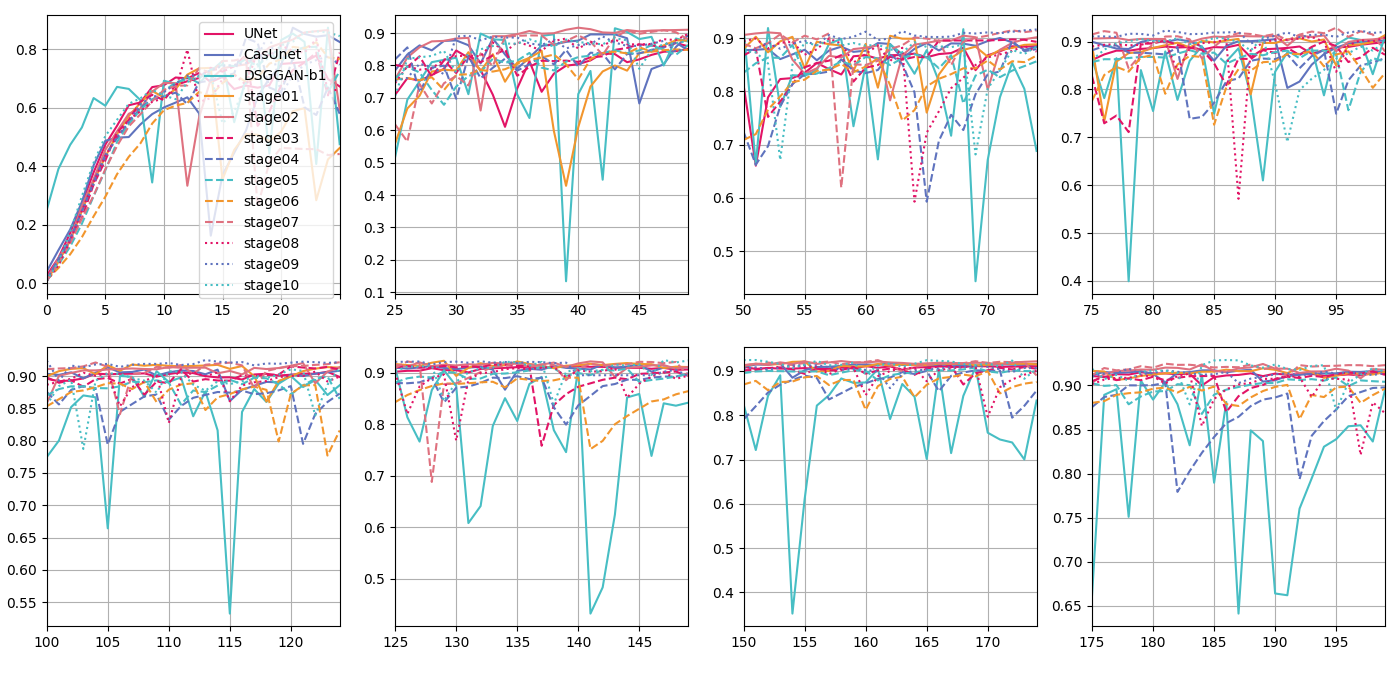
\includegraphics[width=1.0\linewidth]{figures/lung/csvimg_lung_mnv3/ssim_comparison_8.png}
	\caption[ssim]{Evolution of SSIM During Testing Across Epochs. The horizontal axis represents epoch numbers from 0 to 200), and the vertical axis indicates the SSIM values achieved by the model on the test dataset.}
	\label{fig:ssim}
\end{figure*}

Figure \ref{fig:ssim} illustrates SSIM rapidly increasing in initial training (first 25 epochs), stabilizing around 0.9. DSGGAN exhibited fluctuations possibly due to overemphasis on high-dimensional features, but overall SSIM remained high.

\begin{figure}[h]
	\centering
	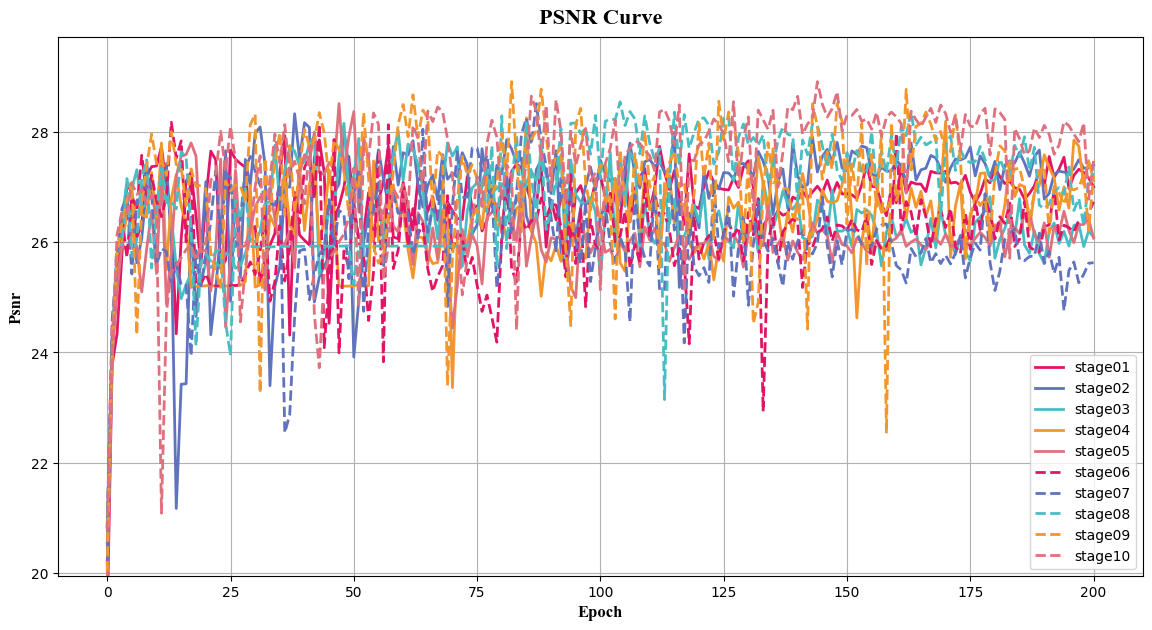
\includegraphics[width=1.0\linewidth]{figures/lung/csvimg_lung_mnv3/psnr_comparison.png}
	\caption[psnr]{Evolution of PSNR During Testing Across Epochs. The horizontal axis represents epoch numbers from 0 to 200, and the vertical axis indicates the PSNR values in dB achieved by the model on the test dataset.}
	\label{fig:psnr}
\end{figure}

PSNR (Figure \ref{fig:psnr}) showed rapid initial improvements with subsequent fluctuations, particularly in 8-, 6-, 4-, and 3-stage models, indicating potential generalization issues with complex data or smaller datasets. Overall, PSNR remained consistently good.

\begin{figure}[h]
	\centering
	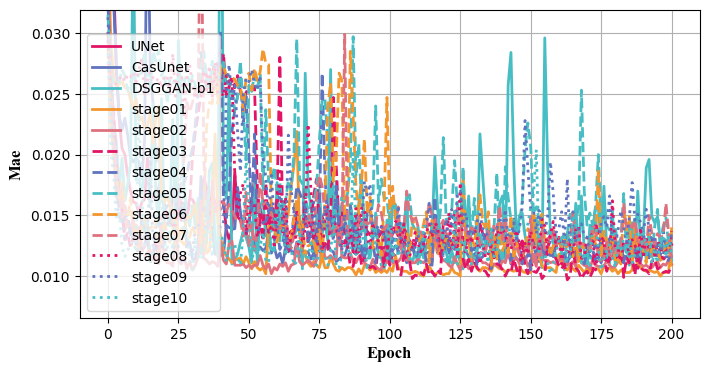
\includegraphics[width=1.0\linewidth]{figures/lung/csvimg_lung_mnv3/mae_comparison.png}
	\caption[mae]{Evolution of MAE During Testing Across Epochs. The horizontal axis represents epoch numbers from 0 to 200, and the vertical axis indicates the MAE values achieved by the model on the test dataset.}
	\label{fig:mae}
\end{figure}

The MAE curve in Figure \ref{fig:mae} declines steeply at the beginning of training, indicating rapid parameter adaptation. Nevertheless, all models converge to uniformly low MAE scores for two principal reasons: (i) the PET intensities are normalized to the [0,1] range, and (ii) dark pixels constitute the majority of each image. Consequently, a well‑trained network quickly discovers that synthesizing images with a disproportionately large share of near‑black pixels is an efficient way to minimize the MAE objective.
Despite these encouraging numbers, a lower MAE does not necessarily translate into superior perceptual quality. Hence, complementary visual‑comparison experiments are required, as purely numerical metrics provide an incomplete—and potentially misleading—assessment of image fidelity.


\begin{figure*}[h]
	\centering
	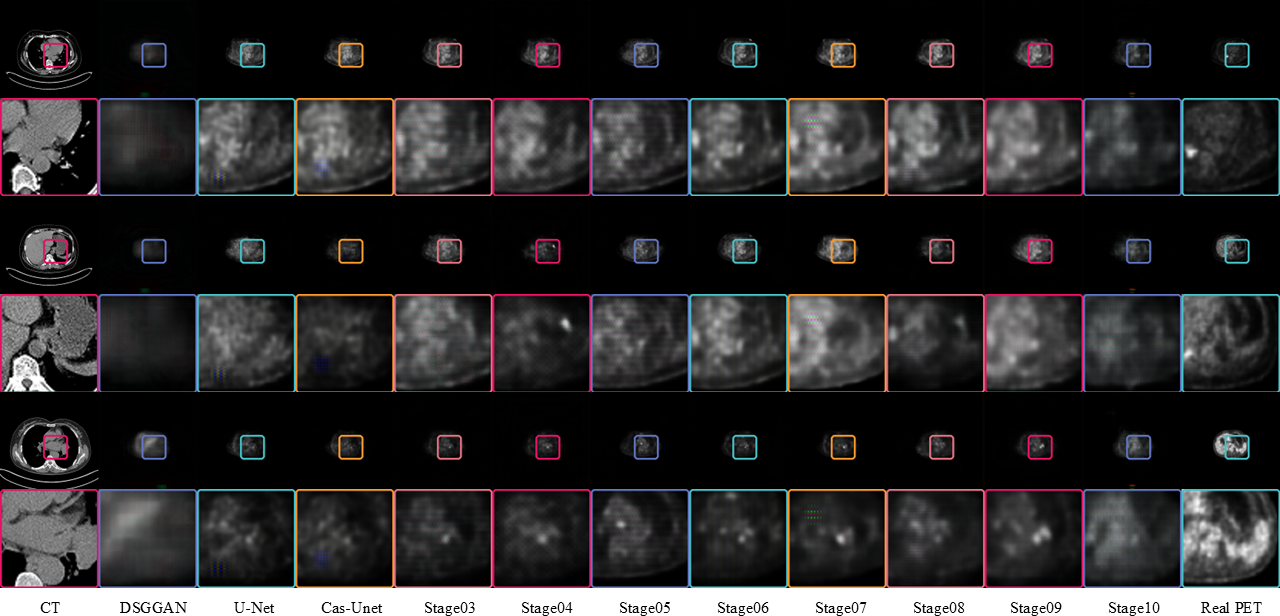
\includegraphics[width=1.0\linewidth]{figures/lung/lung_compare_folder/lung_compare_13.png}
	% \caption[lung_compare]
	\caption[lung_compare]{The figure displayed here showcases PET images generated by various models, compared alongside real CT and PET images. The odd rows present the complete paired PET-CT images, while the even rows provide magnified views of specific regions within these pairs. Each model utilizes the CT image located at the extreme left as the input. The real PET images positioned at the extreme right serve as references for comparison. }
	\label{fig:lung_compare}
\end{figure*}
Visual comparisons (Figure \ref{fig:lung_compare}) indicated pixel-level metrics differed from perceived quality, highlighting artifacts in certain stages due to transpose convolutions. Quantitative metrics did not fully reflect visual quality, underscoring the need for expert evaluations or prior knowledge.
Although the Stage10 and DSGGAN models attained excellent quantitative scores, the images they produced were noticeably blurred. DSGGAN, in particular, exhibited strong numerical performance yet fell short in visual fidelity—a deficiency that may arise from its distinctive skip‑connection design, which can overfit when confronted with complex data or limited sample sizes. These results underscore that pixel‑level metrics alone cannot fully capture perceptual quality; a more comprehensive evaluation that integrates expert judgment or domain‑specific priors is therefore essential. By contrast, the Stage07 network delivered competitive quantitative results while producing images of comparatively higher visual quality. Overall, our proposed frameworks indicate that cascade‑based extensions can achieve robust performance in medical image synthesis, but they also reveal intrinsic limitations that warrant further investigation.

\section{Conclusion}
The proposed cascaded framework effectively enhanced performance and demonstrated stability. Future studies should integrate visual quality assessments and expert evaluations to increase practical utility in medical image translation tasks. The study's findings suggest that the multi-stage cascaded U-Net model can be a valuable tool for medical image synthesis, with potential applications in various medical imaging tasks. The results indicate that the model can effectively learn to generate high-quality images from CT scans, which could aid in improving diagnostic accuracy and treatment planning in clinical settings. Further research is needed to explore the model's performance on larger datasets and its applicability to other imaging modalities.

\section*{Acknowledgements}
We would like to express our sincere gratitude to the National Cancer Institute Cancer Imaging Program for generously making their high-quality medical imaging dataset available and authorized for use on the Internet, providing indispensable resources for the smooth conduct of this research.

\bibliographystyle{unsrt}
% \bibliography{unet_ref}
\bibliography{ref2}

%-------------------------------------------------------------------------
%\nocite{ex1,ex2}
%\bibliographystyle{latex8}
%\bibliography{latex8}

% \begin{thebibliography}{99}
% 	%\addtolength{\itemsep}{-0.8em}
% 	\bibitem{Peter}
% 	Peter. C. Author, ``Paper's name'', Proceeding of ICMLC2002
% 	Conference, Beijing, pp. 111-116, November 2002.

% 	\bibitem{John} John. B. Author, and A. Friend, ``Journal paper's name'', Journal's
% 	name, Vol 39, No. 1, pp. 222-226, Feb. 2001.
% 	\bibitem{Xizhao} Xizhao Wang, His book's name, Publisher, Location, Year.
% \end{thebibliography}




\end{document}
